\chapter{Passive rotation matrices in the 3D Cartesian frame}
\label{Chap:rotations}

As described in the  main text, these are just the transpose of the active 3D rotations.

\vspace{0.2cm}

\noindent\begin{minipage}{0.47\textwidth}
The passive, anticlockwise rotation of a Cartesian reference frame around the axis $\mathbf{x}$ is given in the pre-multiplication matrix form as: 
\begin{equation*}
\mathcal{R}_\mathbf{x}(\theta)=\begin{pmatrix}
1 &  0           & 0 \\
0 & \cos{\theta} & \sin{\theta} \\
0 & -\sin{\theta} & \cos{\theta}
\end{pmatrix}
\label{eq:RotMat}
\end{equation*}
\end{minipage}
\begin{minipage}{0.5\textwidth}
\centering
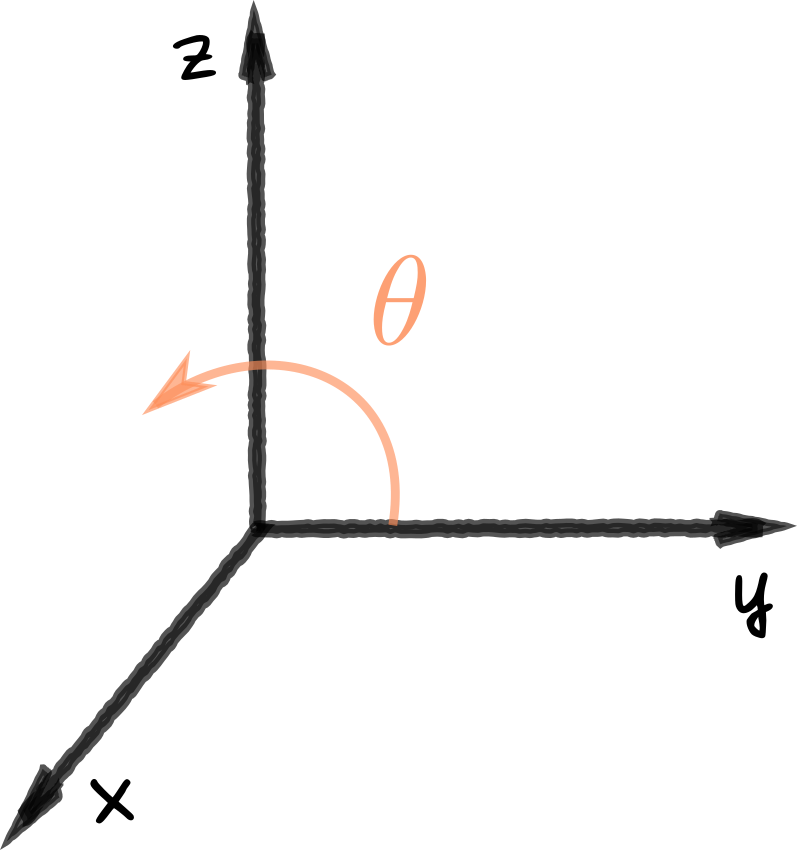
\includegraphics[width=0.45\linewidth]{Figures/Rx.png}
\captionof*{figure}{Basic rotation around $\mathbf{x}$.}
\end{minipage}



\noindent\begin{minipage}{0.47\textwidth}
The passive, anticlockwise rotation of a Cartesian reference frame around the axis $\mathbf{y}$ is given in the pre-multiplication matrix form as: 
\begin{equation*}
\mathcal{R}_\mathbf{y}(\theta)=\begin{pmatrix}
\cos{\theta}  &  0     & -\sin{\theta} \\
0             & 1      & 0 \\
\sin{\theta} & 0      & \cos{\theta}
\end{pmatrix}
\end{equation*}
\end{minipage}
\begin{minipage}{0.5\textwidth}
\centering
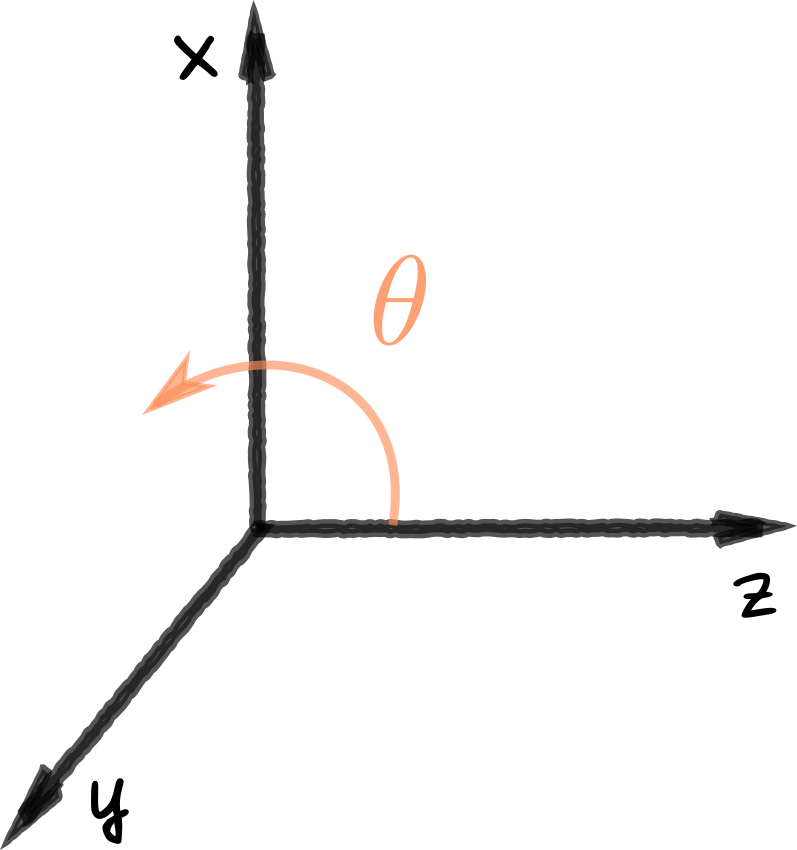
\includegraphics[width=0.45\linewidth]{Figures/Ry.png}
\captionof*{figure}{Basic rotation around $\mathbf{y}$.}
\end{minipage}



\noindent\begin{minipage}{0.47\textwidth}
The passive, anticlockwise rotation of a Cartesian reference frame around the axis $\mathbf{z}$ in the pre-multiplication matrix form is: 
\begin{equation*}
\mathcal{R}_\mathbf{z}(\theta)=\begin{pmatrix}
\cos{\theta} & \sin{\theta} & 0 \\
-\sin{\theta} & \cos{\theta}  & 0 \\
0            &  0            & 1
\end{pmatrix}
\end{equation*}
\end{minipage}%
\begin{minipage}{0.5\textwidth}
\centering
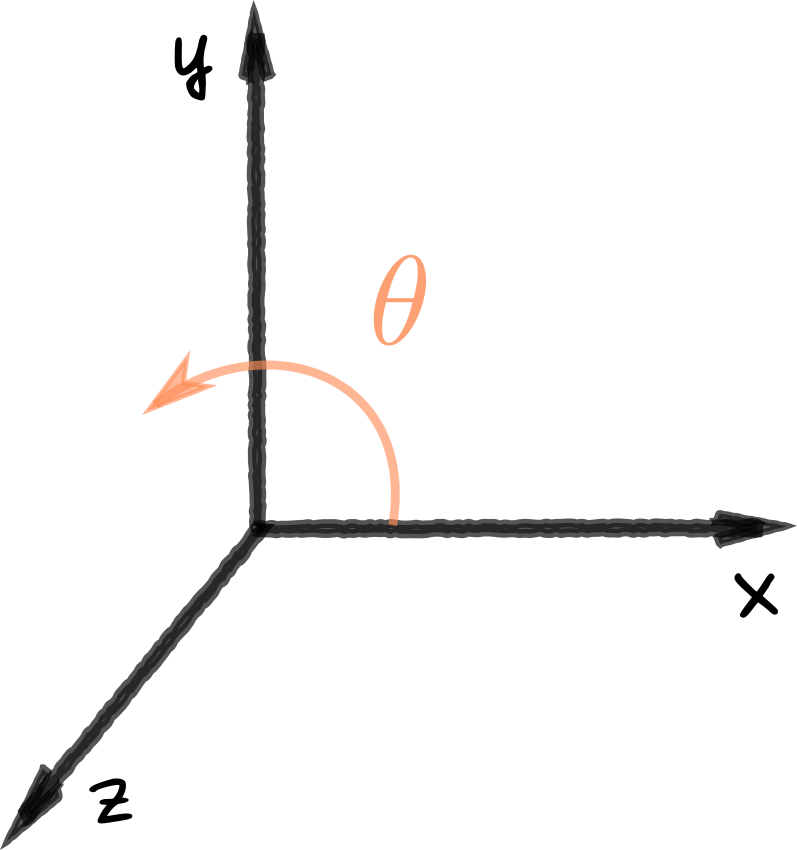
\includegraphics[width=0.45\linewidth]{Figures/Rz.png}
\captionof*{figure}{Basic rotation around $\mathbf{z}$.}
\end{minipage}

